%	현대물리실험 보고서
%	실험5
%	202100973 이승엽

%----------------------------------------------------------------------------------------
%	PACKAGES AND DOCUMENT CONFIGURATIONS
%----------------------------------------------------------------------------------------

\documentclass[a4paper, 10pt, nanum]{CSUniSchoolLabReport}
% use UTF8 encoding
\usepackage[utf8]{inputenc}
% use KoTeX package for Korean
\usepackage{kotex}
% use ams' math font
\usepackage{amsmath}
\usepackage{hyperref}
% use table
\usepackage{graphicx}
\usepackage{multirow}
\usepackage{indentfirst}
\usepackage{setspace}
\usepackage{enumitem}
\usepackage{wrapfig}
\usepackage{epstopdf}
% use captions
\usepackage{caption}
\usepackage{subcaption}
\usepackage{blindtext}
% package crucial to implement colors 
\usepackage{xcolor}
% use tikz 
\usepackage{tikz}
% use layout frame
% \usepackage{showframe}
% Use a package that puts your Python code.
\usepackage[cache=false]{minted}

% Setting the graphics path
\graphicspath{{Figures/}}

% % only for show page layout
% \renewcommand\ShowFrameLinethickness{0.25pt}
% \renewcommand*\ShowFrameColor{\color{red}}

\setlength{\parindent}{0.2in} % 들여쓰기 길이 설정
\setlength{\parskip}{3mm} % 문단 간의 간격 조절
\setstretch{1.5} % 줄간격
% \graphicpath{{Figures/}} % fig 경로 설정

\addbibresource{reference.bib} % Bibliography file (located in the same folder as the template)

%----------------------------------------------------------------------------------------
%	REPORT INFORMATION
%----------------------------------------------------------------------------------------

\title{현대물리실험 실험5 보고서 \\ 전자의 회절 및 XRD} % Report title

\author{\textsc{Department of Physics} 202100973 이승엽}

\date{\today}

%----------------------------------------------------------------------------------------

\begin{document}

\maketitle % Insert the title, author and date using the information specified above

\begin{center}
	\begin{tabular}{l r}
		Date Performed: & May 30, 2023 \\ % Date the experiment was performed
		Partners: & 202100969 이규리 \\ % Partner names
		& 202100989 한누리 \\
		Instructor: & Professor 이기주 \\ % Instructor/supervisor
		Typesetting: & LaTeX \\
		Datafitting: & OriginLab \& Python \\
	\end{tabular}
\end{center}

%----------------------------------------------------------------------------------------
%	ABSTRACT
%----------------------------------------------------------------------------------------

\maketitle
% \begin{abstract}
% 	This report ...
% \end{abstract}

%----------------------------------------------------------------------------------------
%	INTRODUCTION
%----------------------------------------------------------------------------------------

\section{Introduction}

\begin{enumerate}[label=\arabic*.]
	\item 전자의 회절 격자에 대해 조사한다.
	\item 회절 무늬를 관측하여 흑연의 interplanar spacing을 측정한다.
	\item X-선을 사용하여 브래그 각을 측정하고, 그 특성 동 선의 에너지 값을 계산하고, 비교한다.
\end{enumerate}



%----------------------------------------------------------------------------------------
%	THEORY
%----------------------------------------------------------------------------------------

\section{Theory}

	파동으로서의 전자 : 운동량 $P$를 갖고 있는 전자의 파장은 드브로이 방정식에 의하면
	\begin{align}
		\lambda = \frac{h}{P}
	\end{align}
	이다. 또 운동량 p는 전자를 가속한 전압이 V라 할 때 운동 에너지의 식에서부터 구할 수 있다.
	\begin{align}
		K = \frac{P^2}{20} = eV
	\end{align}
	로 두 수식을 연립하면
	\begin{align}
		\lambda = \frac{h}{\sqrt{2meV}}
	\end{align}
	가 된다. 참고로 여기서 사용되는 전압 범위에서는 상대론적 질량과 고전적인 질량의 차이는 0.5\% 보다 작다.

	회절 무늬: 전자가 구리(금속입자:Cu) grating에 입혀진 다결정 흑연박막에 부딪치면 브레그 조건에 따라 반사된다. $n$이 자연수 1, 2, 3, ...일 때,
	\begin{align}
		n\lambda = 2d \sin\theta
	\end{align}
	가 된다.

	흑연 결정의 구조와 회절격자 사이의 거리는 Fig. 1, 2와 같다
	\begin{figure}[ht!]
		\centering
		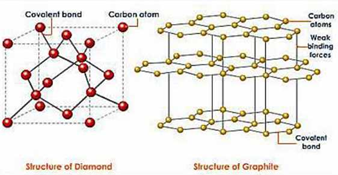
\includegraphics[width=5cm]{Figures/diamond-graphite.png}
		\caption{다이아몬드와 흑연 결정(graphite)의 구조 차이.}
		\label{fig:diamond-graphite}
	\end{figure}
	\begin{figure}[ht!]
		\centering
		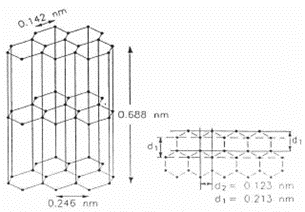
\includegraphics[width=5cm]{Figures/graphite.png}
		\caption{흑연 격자 간 거리.}
		\label{fig:graphite}
	\end{figure}

	다결정 측연에서는 각각의 층(layer)사시의 결합(bond)이 깨져서 그 방향이 제멋대로이다. 따라서 전자빔(또는 전자선)은 원뿔모양의 cone처럼 퍼져서 진행하며 회절무늬를 형광판에 원으로 나타난다. 브래그각 $\theta$는 원 모양의 회절 무늬의 반지름에서 측정할 수 있다. (단, Fig. 3에서 원의 특성에 의해 $\alpha = 2\theta$임을 알고 있어야 한다.)
	\begin{figure}[ht!]
		\centering
		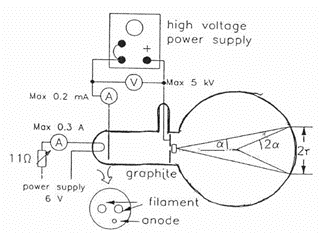
\includegraphics[width=5cm]{Figures/experiment.png}
		\caption{실험장치의 개략도.}
		\label{fig:experiment}
	\end{figure}
	따라서
	\begin{align}
		\sin 2\alpha = \frac{D_n}{R}
	\end{align}
	이 된다. 여기서 $R$은 유리 전구의 반지름으로 $2R = L$.이다. 만약 $\alpha$가 매우 작다면 삼각함수의 특성에 의해
	\begin{align}
		D_n = \frac{2Rn\lambda}{d}
	\end{align}

	XRD 분석이란 X-ray를 원하는 시편에 회절 시켜 시편의 내부 정보를 그래프로 나타내는 분석법이다. 보통 최종 결과물은 아래의 그림 그래프와 같다. X축은 $2\theta$로 Y축은 intensity라는 값으로 그래프로 나타내며 여러 상들의 고유한 각도에서 peak값이 나타나 시편 속에 어떠한 phase로 이루어져 있는지 확인할 수 있는 분석 방법이다.
	\begin{figure}[ht!]
		\centering
		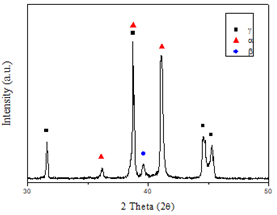
\includegraphics[width=5cm]{Figures/exam_xrd.png}
		\caption{}
		\label{fig:exam_xrd}
	\end{figure}

%----------------------------------------------------------------------------------------
%	EXPERIMENTAL METHOD
%----------------------------------------------------------------------------------------

\section{Experimental Method}

\subsection*{실험1. 전자의 회절}

	\begin{figure}[ht!]
		\centering
		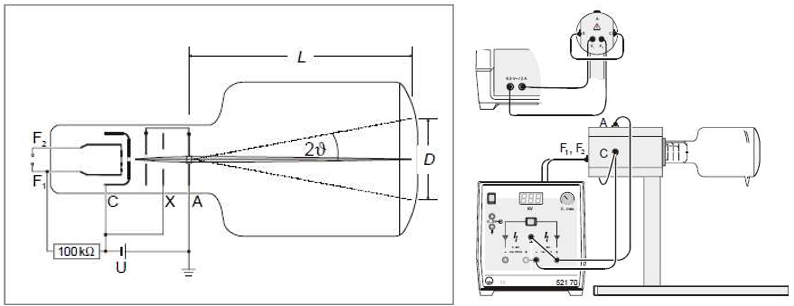
\includegraphics[width=8cm]{Figures/experimental_exam.png}
		\caption{}
		\label{fig:experimental_exam}
	\end{figure}
	\begin{enumerate}[label=\arabic*.]
		\item F1과 F2를 110V 전용 high-voltage power supply로 10 kV 걸어준다.
		\item C와 X 커넥터를 주황색 power supply의 음극에 연결한다.
		\item A 커넥터를 주황색 power supply의 양극에 연결한다.
		\item 주황색 power supply의 전압을 서서히 올려준다. (이 전압을 accelerating voltage $U$라고 한다.)
		\item Accelerating voltage $U$를 2 kV에서 5 kV까지 0.5 kV간격으로 올려주며 스크린에 비춘 원형고리의 지름 $D_1$과 $D_2$를 버니어 켈리퍼스로 측정한다.
	\end{enumerate}
	\begin{figure}[ht!]
		\centering
		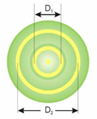
\includegraphics[height=5cm]{Figures/experimental_exam2.png}
		\caption{}
		\label{fig:experimental_exam2}
	\end{figure}

\subsection*{실험2. XRD}

	\begin{enumerate}[label=\arabic*.]
		\item 셋팅되어 있는 XRD 기기와 데이터 프로그램 measure을 실행한다.
		\item 결정립 LiF, KBr을 측정할 것이다.
		\item 1:2 coupling mode, Gate time 2 s; angle step width 0.1 degree로 한다.
		\item Scanning range from 4 to 55 degree (LiF), and from 3 to 75 degree (KBr).
		\item Anode voltage 35 kV; anode current 1 mA.
		\item 양자화되어 있는 에너지 준위를 계산한다.		
	\end{enumerate}

%----------------------------------------------------------------------------------------
%	RESULT AND DISCUSSION
%----------------------------------------------------------------------------------------

\section{Result and Discussion}

\subsection*{실험1. 전자의 회절}

	\begin{table}[ht!]
		\label{tab:2}
		\centering
		\caption{Accelerating voltage $U$에 따른 회절 지름}
		\resizebox{\textwidth}{!}{
		\begin{tabular*}{\textwidth}{@{\extracolsep{\fill}}ccc|ccc}
				\noalign{\smallskip}\noalign{\smallskip}\hline\hline
				& $U$ (kV) & & $D_1$ (cm) & $D_2$ (cm) \\
			\hline
				& 3.5 & & 2.90 & 4.78 \\
				& 4.0 & & 2.75 & 4.55 \\
				& 4.5 & & 2.66 & 4.26 \\
				& 5.0 & & 2.51 & 4.00 \\
				& 5.5 & & 2.42 & 3.73 \\
				& 6.0 & & 2.24 & 3.47 \\
				& 6.5 & & 2.24 & 3.27 \\
			\hline
			\hline
		\end{tabular*}
		}
	\end{table}

	\begin{figure}[ht!]
		\centering
		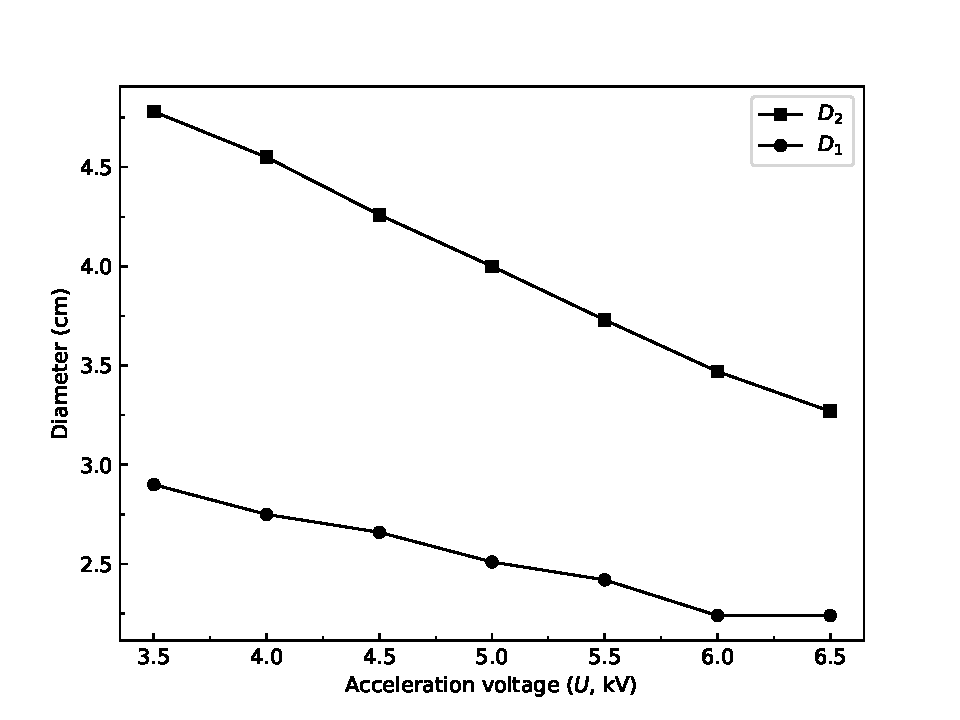
\includegraphics[width=8cm]{Figures/graph1.pdf}
		\caption{}
		\label{fig:graph1}
	\end{figure}

	가속 전압이 올라갈수록 회절 지름이 선형적으로 감소함을 보인다. 이때, $D_2$가 $D_1$보다 크게 줄어든다.


\subsection*{실험2. XRD}
	
	\begin{figure}[ht!]
		\centering
		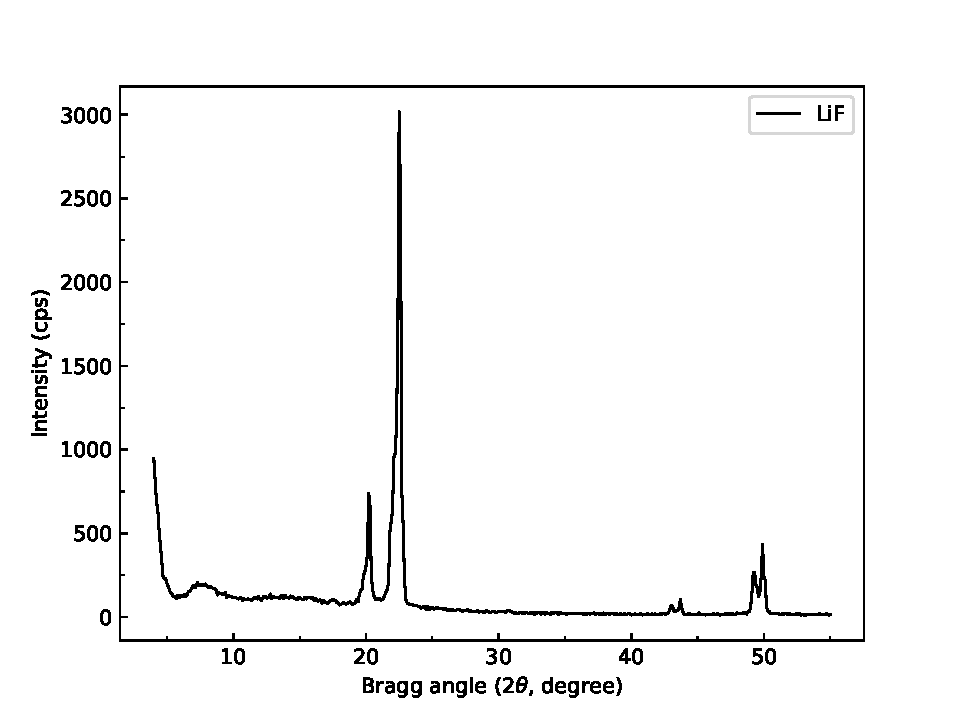
\includegraphics[width=8cm]{Figures/graph2-1.pdf}
		\caption{}
		\label{fig:graph2-1}
	\end{figure}

	\begin{figure}[ht!]
		\centering
		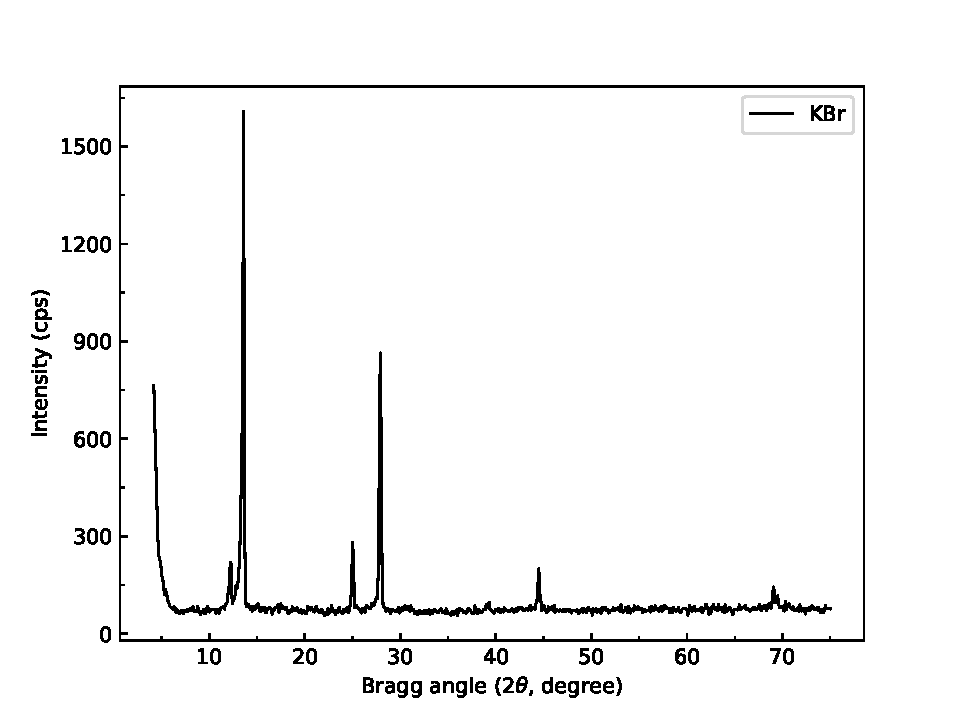
\includegraphics[width=8cm]{Figures/graph2-2.pdf}
		\caption{}
		\label{fig:graph2-2}
	\end{figure}

	\begin{table}[ht!]
		\label{tab:3}
		\centering
		\caption{}
		\resizebox{\textwidth}{!}{
		\begin{tabular*}{\textwidth}{@{\extracolsep{\fill}}cccc|ccc}
				\noalign{\smallskip}\noalign{\smallskip}\hline\hline
				\multicolumn{4}{c|}{LiF} & \multicolumn{2}{c}{KBr} \\
				& $2\theta$ (degree) & FWHM & & $2\theta$ (degree) & FWHM \\
			\hline
				& 20.2 & 0.26981 & & 12.2 & 0.24536 \\
				& 22.5 & 0.41468 & & 13.6 & 0.16384 \\
				& 42.1 & 2.86019 & & 25.0 & 0.19983 \\
				& 43.9 & 6.21849E-4 & & 27.9 & 0.24018 \\
				& 49.3 & 0.44567 & & 39.1 & 0.57649 \\
				& 49.9 & 0.34325 & & 44.5 & 0.24495 \\
				& 		 &				 & & 69.2 & 0.71129 \\
			\hline
			\hline
		\end{tabular*}
		}
	\end{table}

	Table 2에 따라 에너지 레벨에 맞춰 peak가 생김을 알 수 있다.



%----------------------------------------------------------------------------------------
%	CONCLUSIONS
%----------------------------------------------------------------------------------------

\section{Conclusions}

	실험1은 에너지에 따라 회절이 많이 됨을 알 수 있다. 실험2는 X-ray를 쏘아 각도에 따라 물질마다 에너지 레벨이 보임을 알 수 있다.


%----------------------------------------------------------------------------------------
%	SOURCE CODE FOR PYTHON FITTING
%----------------------------------------------------------------------------------------

\section{Source code for Python fitting}

\definecolor{LightGray}{gray}{0.97}
% minted option fontsize=\footnotesize, 

\begin{listing}[ht!]
	\begin{minted}[breaklines=true, mathescape, frame=lines,	framesep=2mm,	baselinestretch=1.2,	bgcolor=LightGray,	fontsize=\footnotesize,	linenos]{python}
import matplotlib.pyplot as plt
import matplotlib.ticker as tck
import numpy as np
from numpy import genfromtxt
from matplotlib.ticker import MultipleLocator, IndexLocator, FuncFormatter, FormatStrFormatter
from matplotlib.dates import MonthLocator, DateFormatter
from matplotlib.transforms import Bbox

# Data1
data = genfromtxt('data1.csv', delimiter=',', encoding='UTF8', dtype=float)
## 모든(:) column=0, 1, 2에 대해 row=0, 1, 2을 출력
X = data[:, 0]
Y1 = data[:, 1]
Y2 = data[:, 2]

# Figure
fig, ax = plt.subplots()
plt.plot(X, Y2, label='$D_2$', color='k', marker='s', markersize=5, linestyle='solid', linewidth=1)
plt.plot(X, Y1, label='$D_1$', color='k', marker='o', markersize=5, linestyle='solid', linewidth=1)
plt.xlabel('Acceleration voltage ($U$, kV)')
plt.ylabel('Diameter (cm)')

# Place a legend on the Axes. (location=0='best')
plt.legend(loc=0)

# Figure tick setting
plt.tick_params(axis='x', labelsize=10, direction='in')
plt.tick_params(axis='y', labelsize=10, direction='in')
ax.tick_params(axis='x', which='minor', bottom=True, direction='in')
ax.tick_params(axis='y', which='minor', left=True, direction='in')
## x값이 n의 배수일 때마다 메인 눈금 표시
ax.xaxis.set_major_locator(MultipleLocator(.5)) 
ax.yaxis.set_major_locator(MultipleLocator(.5))
## 메인 눈금이 표시될 형식
ax.xaxis.set_major_formatter('{x}')
ax.yaxis.set_major_formatter('{x}')
## 서브 눈금은 x값이 n의 배수인 경우마다 표시
ax.xaxis.set_minor_locator(MultipleLocator(.25)) 
ax.yaxis.set_minor_locator(MultipleLocator(.25))

# Plot show
plt.show()
	\end{minted}
	\caption{Example from external file}
	\label{listing:graph1-code}
\end{listing}

\begin{listing}[ht!]
	\begin{minted}[breaklines=true, mathescape, frame=lines,	framesep=2mm,	baselinestretch=1.2,	bgcolor=LightGray,	fontsize=\footnotesize,	linenos]{python}
import matplotlib.pyplot as plt
import matplotlib.ticker as tck
import numpy as np
from numpy import genfromtxt
from matplotlib.ticker import MultipleLocator, IndexLocator, FuncFormatter
from matplotlib.dates import MonthLocator, DateFormatter

# Data2-1
data = genfromtxt('data2-1.csv', delimiter=',', encoding='UTF8')
## from row=3 to infty, column=0에 대해 row=0을 출력
X = data[3:, 0]
## from row=3 to infty, column=1에 대해 row=1을 출력
Y = data[3:, 1]

# Figure
fig, ax = plt.subplots()
plt.plot(X, Y, label='LiF', color='k', linestyle='solid', linewidth=1)

# Figure title
plt.xlabel('Bragg angle (2$\\theta$, degree)')
plt.ylabel('Intensity (cps)')

# figure tick setting
plt.tick_params(axis='x', labelsize=10, direction='in')
plt.tick_params(axis='y', labelsize=10, direction='in')

# Place a legend on the Axes. (location=0='best')
plt.legend(loc=0)

# figure minor tick setting
ax.tick_params(axis='x', which='minor', bottom=True, direction='in')
ax.tick_params(axis='y', which='minor', left=True, direction='in')
## x값이 5의 배수일 때마다 메인 눈금 표시
ax.xaxis.set_major_locator(MultipleLocator(10)) 
ax.yaxis.set_major_locator(MultipleLocator(500))
## 메인 눈금이 표시될 형식
ax.xaxis.set_major_formatter('{x:.0f}')
ax.yaxis.set_major_formatter('{x:.0f}')
## 서브 눈금은 x값이 n의 배수인 경우마다 표시
ax.xaxis.set_minor_locator(MultipleLocator(5)) 
ax.yaxis.set_minor_locator(MultipleLocator(250))

# Plot show
plt.show()
	\end{minted}
	\caption{Example from external file}
	\label{listing:graph2-code}
\end{listing}


\begin{listing}[ht!]
	\begin{minted}[breaklines=true, mathescape, frame=lines,	framesep=2mm,	baselinestretch=1.2,	bgcolor=LightGray,	fontsize=\footnotesize,	linenos]{python}
import matplotlib.pyplot as plt
import matplotlib.ticker as tck
import numpy as np
from numpy import genfromtxt
from matplotlib.ticker import MultipleLocator, IndexLocator, FuncFormatter
from matplotlib.dates import MonthLocator, DateFormatter

# Data2-2
data = genfromtxt('data2-2.csv', delimiter=',', encoding='UTF8')
## from row=15 to infty, column=0에 대해 row=0을 출력
X = data[15:, 0]
## from row=15 to infty, column=1에 대해 row=1을 출력
Y = data[15:, 1]

# Figure
fig, ax = plt.subplots()
plt.plot(X, Y, label='KBr', color='k', linestyle='solid', linewidth=1)

# Figure title
plt.xlabel('Bragg angle (2$\\theta$, degree)')
plt.ylabel('Intensity (cps)')

# figure tick setting
plt.tick_params(axis='x', labelsize=10, direction='in')
plt.tick_params(axis='y', labelsize=10, direction='in')

# Place a legend on the Axes. (location=0='best')
plt.legend(loc=0)

# figure minor tick setting
ax.tick_params(axis='x', which='minor', bottom=True, direction='in')
ax.tick_params(axis='y', which='minor', left=True, direction='in')
## x값이 5의 배수일 때마다 메인 눈금 표시
ax.xaxis.set_major_locator(MultipleLocator(10)) 
ax.yaxis.set_major_locator(MultipleLocator(300))
## 메인 눈금이 표시될 형식
ax.xaxis.set_major_formatter('{x:.0f}')
ax.yaxis.set_major_formatter('{x:.0f}')
## 서브 눈금은 x값이 n의 배수인 경우마다 표시
ax.xaxis.set_minor_locator(MultipleLocator(5)) 
ax.yaxis.set_minor_locator(MultipleLocator(150))

# Plot show
plt.show()
	\end{minted}
	\caption{Example from external file}
	\label{listing:graph3-code}
\end{listing}

%----------------------------------------------------------------------------------------
%	BIBLIOGRAPHY
%----------------------------------------------------------------------------------------

% \printbibliography % Output the bibliography

%----------------------------------------------------------------------------------------

\end{document}